\begin{figure*}[t]
\centering
\vspace{-2mm}
 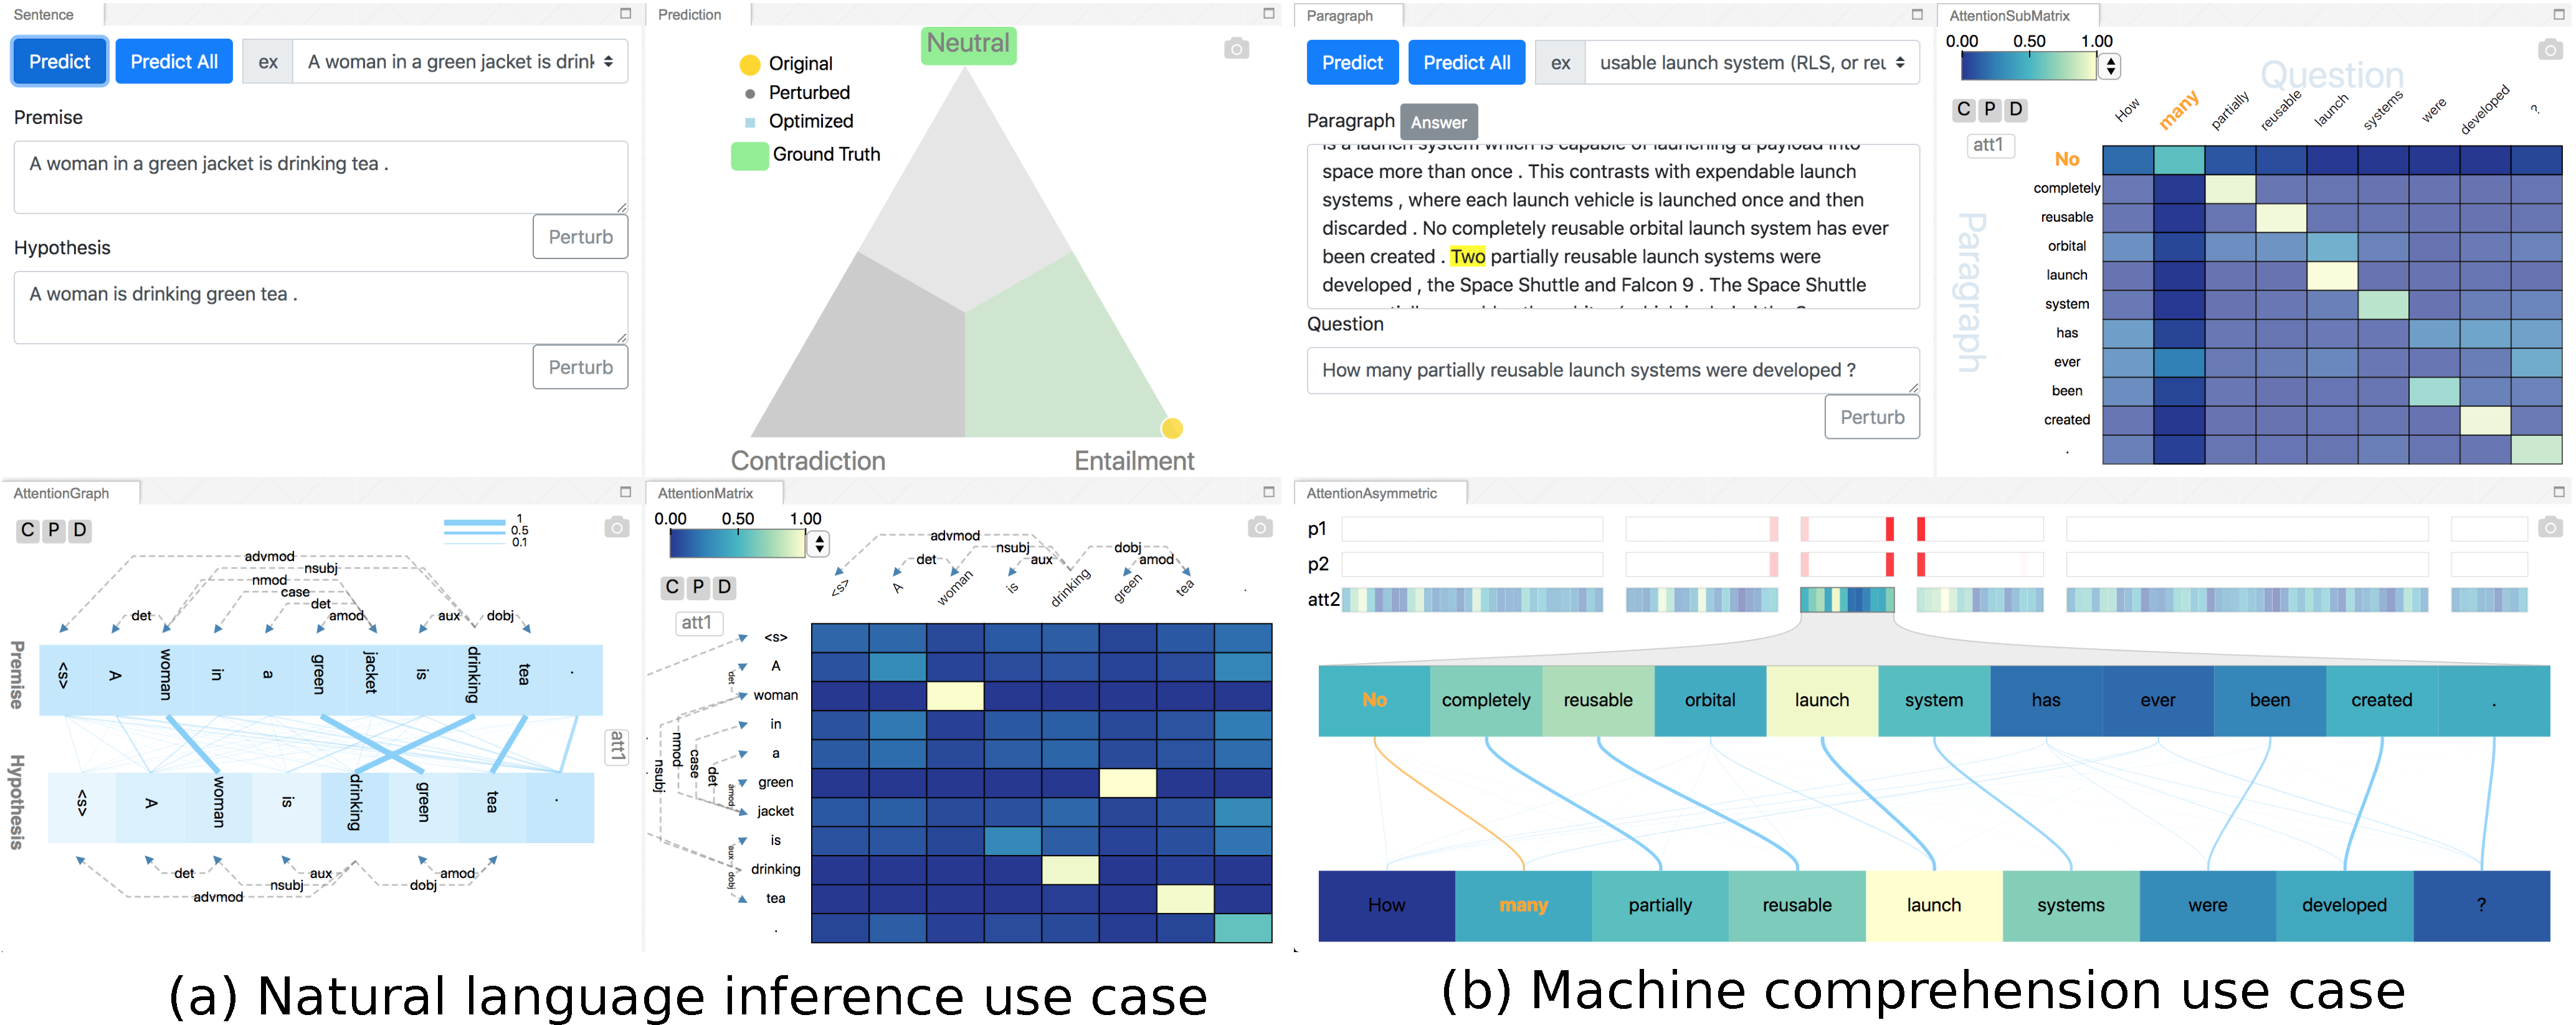
\includegraphics[width=1.0\linewidth]{NLI_MC_interface}
  \vspace{-6mm}
 \caption{
Illustration of different configurations for the natural language inference and machine comprehension tasks.
}
\label{fig:pipelineUpdate}
\end{figure*}

\section{Application}


\subsection{Natural Language Inference}
We demonstrate our visualization system on the decomposable attention networks
for NLI task. The goal is that, given a premise sentence and a hypothesis sentence,
predict their relation as one of \emph{Entailment, Contradiction, Neutral}.
The model can be formalized as the following:
\begin{align}
	P^\prime, H^\prime &= f(P), f(H)\\
	\overleftarrow{A} &= P^\prime \cdot H^\prime\\
	\overrightarrow{A} &= H^\prime \cdot P^\prime\\
	y &= g(P, H, P^\prime, H^\prime, \overleftarrow{A}, \overrightarrow{A})
\end{align}
where $P$ and $H$ are input embedding matrices for the premise and the hypothesis, $\overleftarrow{A}$
and $\overrightarrow{A}$ are attentions, and $y$ is the predicted probabilities for candidate classes.
Our system visualized the bidirectional attentions and their interaction with output distribution over labels.


\subsection{Machine Comprehension}
In machine comprehension task, two sequences of texts are given: context and question.
The target is to select a span of text from the context that answers the question. We provide a simple model
formulation and refer the reader to the paper for details.
\begin{align}
	C^\prime, Q^\prime &= BiLSTM(C), BiLSTM(Q)\\
	\overleftarrow{A} &= u(C^\prime, Q^\prime)\\
	\overrightarrow{A} &= v(C^\prime, Q^\prime)\\
	s &= m(C^\prime, Q^\prime, \overleftarrow{A}, \overrightarrow{A})\\
	e &= n(s, C^\prime, Q^\prime, \overleftarrow{A}, \overrightarrow{A})
\end{align}
where $C$ and $Q$ are embedding matrices for the context and the question,
$\overleftarrow{A}$ and $\overrightarrow{A}$ are bidirectional attention flows,
$s$ and $e$ are probabilities for starting and ending indices of the answer span.
Our system reveals the internal states of $\overleftarrow{A}$, $\overrightarrow{A}$,
$s$ and $e$.
